\documentclass[11pt]{article}
\usepackage{graphicx}
\usepackage{amsmath,amssymb,amstext}
\usepackage{listings}
\usepackage{xcolor}

\definecolor{codegreen}{rgb}{0,0.6,0}
\definecolor{codegray}{rgb}{0.5,0.5,0.5}
\definecolor{codepurple}{rgb}{0.58,0,0.82}
\definecolor{backcolour}{rgb}{0.95,0.95,0.92}

\lstdefinestyle{mystyle}{
    backgroundcolor=\color{backcolour},   
    commentstyle=\color{codegreen},
    keywordstyle=\color{magenta},
    numberstyle=\tiny\color{codegray},
    stringstyle=\color{codepurple},
    basicstyle=\ttfamily\footnotesize,
    breakatwhitespace=false,         
    breaklines=true,                 
    captionpos=b,                    
    keepspaces=true,                 
    numbers=left,                    
    numbersep=5pt,                  
    showspaces=false,                
    showstringspaces=false,
    showtabs=false,                  
    tabsize=2
}

\lstset{style=mystyle}
 
\title{NURBS}
\author{Justin Unger}
\date{\today{}, Mosbach} 
 
\begin{document}
\maketitle
\tableofcontents

\section{Einleitung}
\label{sec:einleitung}
Produkte haben eine Vielzahl von Phasen, welche sie durchlaufen, bis sie in die Produktion kommen.
Besonders bei Autos ist das Design sehr wichtig.
Um so komplexe Formen zu generieren, gibt es verschiedene Möglichkeiten.
Wenn diese digital modelliert werden, dann müssen diese im Hintergrund mathematisch dargestellt werden. 

In dieser Ausarbeitung wird ein Standardverfahren für diese Mathematische Darstellung vorgestellt: \emph{NURBS}.
NURBS steht für Non-uniform rational B-Splines. 
Was diese einzelnen Bestandteile der Abkürzung mit dem Modell zu tun haben, wird im Laufe der Arbeit vorgestellt.

Bevor dies geschehen kann, müssen explizit zwei Vorbetrachtungen zu rate gezogen werden: die \emph{Bézier-Kurven} und die \emph{Tensor Produkt Oberflächen}.
Dahingehend wird auch der Rationale Aspekt erläutert.

Anschließend werden im Abschnitt  \emph{\ref{sec:definitionnurbs} Definition NURBS} die weiteren Bestandteile von NURBS dargestellt.
Dabei werden auch B-Splines für sich selbst vorgestellt.

Im Kapitel \emph{\ref{sec:modellierung} Modellierung} wird beispielhaft gezeigt, wie in einem Programm mit den NURBS gearbeitet werden kann. 
Diese Kapitel ist explizit nicht mathematisch. 
Es soll die Anwendung für Designer und nicht für Mathematiker darstellen. 

Diese Arbeit basiert auf den \emph{NURBS Book} von Les Piegl und Wayne Tille. 
Wenn eine andere Quelle verwendet wird, ist diese Referenziert.
Ansonsten ist dieses Buch die Hauptquelle, bei welcher alle (nicht anders markierte Formeln) übernommen wurden. 

\section{Vorbetrachtung}
\label{sec:vorbetrachtung}
\subsection{Bézier-Kurven}
\label{sec:bezierkurven}

Pierre Etienne Bézier arbeitete bei Renault. 
Dabei hat er eine mathematische Beschreibung für beliebige Kurven gefunden, welche sich anhand von Kontrollpunkten definieren lassen.
Dabei muss die Kurve (Bézier-Kurve) nicht durch jeden Kontrollpunkt verlaufen. 
Dennoch wird die Form durch die Kontrollpunkte definiert.

\begin{figure}[h]
 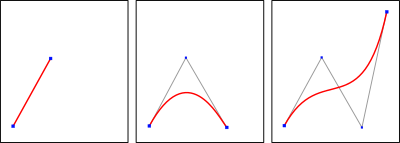
\includegraphics{./pictures/Bezier_grad123.png}
\caption{Bezier-Kurven vom 1. bis 3. Grad}
\label{abb:bezierkurven123}
\end{figure}

Eine Bézier-Kurve hat immer einen bestimmten Grad \emph{n}. 
Zudem hat sie \emph{n+1} Kontrollpunkte P.

\begin{equation}
 C(u) = \sum_{i=0}^{n} B_{i,n} (u) * P_{i}
\end{equation}

\begin{equation}
 B_{i,n} (u) = \frac{n!}{i!*(n-i)!} * u^{i} * (1-u)^{n-i}
\end{equation}

\begin{equation}
 0 \leq u \leq 1
\end{equation}

Mit diesen Gleichungen lassen sich viele zwei dimensionale Formen darstellen.  
Jedoch nicht alle.
Bézier-Kurven sind eine andere Darstellung für Polynome. 
Die "Grunddarstellung" von Polynomen sind: 
 \begin{equation}
x(u) = a_{0} * u^{0} + a_{1} * u^{1} + a_{2} * u^{2} + ... + a_{n} * u^{n}
\end{equation}

\begin{equation}
x(u) = b_{0} * u^{0} + b_{1} * u^{1} + b_{2} * u^{2} + ... + b_{n} * u^{n}
\end{equation}

Diese können jedoch keine Kreise, Ellipsen oder Hyperbeln exakt darstellen. 
Dazu sind gebrochen rationale Polynome (Englisch: rational polynomes) notwendig. 

\begin{equation}
x(u) = \frac{X(u)}{W(u)}
\end{equation}

\begin{equation}
y(u) = \frac{Y(u)}{W(u)}
\end{equation}
Wenn Bézier-Kurven  gebrochen rationale Polynome darstellen sollen, kann folgende die Gleichung  verwendet werden.
Die Funktion $B(u)$ ist die gleiche wie bei rationalen Bézier-Kurven.

\begin{equation}
C(u) = \sum_{i=0}^{n} R_{i,n} (u) * u_{i} * P_{i}
\end{equation}

\begin{equation}
R_{i,n} (u) = \frac{B_{i,n} (u) * w_{i}}{\sum_{j=0}^{n} B_{j,n} (u) * w_{j}}
\end{equation}

\begin{equation}
B_{i,n} (u) = \frac{n!}{i! * (n-i)!} * u^{i} * (1-u)^{n-i}
\end{equation}

Bei $C(u)$ ist der Aufbau auch gleich, außer das $B_{i,n}(u)$ durch $R_{i,n}(u)$ ersetzt wurde. 
Die Funktion  $R_{i,n}(u)$ ist der Bruch der Funktion. 
Dieser stellt das Verhältnis zwischen dem aktuellen Punkt und der Summe aller Punkte dar. 
Der Parameter $w_{i}$ stellt die Gewichtung dar. 
Wenn die Abbildung \ref{abb:bezierkurven123} erneut betrachtet, kann die Gewichtung als Einflussstärke eines Kontrollpunktes verstanden werden. 

Da die Gleichung für Bézier-Kurven immer identisch ist, kann jede mögliche Kurve durch zwei Listen darstellt werden.
Eine Liste mit den Kontrollpunkten und eine Liste mit den Gewichtungen für die Punkte. 
Da jedoch dann immer beachtet werden muss, das beide Listen gleich groß sind, wird eine weitere Darstellungsmöglichkeit für die Punkte gewählt.
Dabei werden die Punkte um eine Dimension erweitert. 
Zwei dimensionale Punkte werden zu drei dimensionalen Punkten.

\begin{equation}
P = (x,y)
\end{equation}

\begin{equation}
P^w = (w*x, w*y, w)
\end{equation}

\begin{equation}
H\{P^w\} = P
\end{equation}

Dadurch ist die Gewichtung direkt mit im Punkt mit angegeben. 
Diese Umwandlung nennt sich Homogene Koordinaten. 
Die Geometrische Bedeutung ist das Zuweisen (Mappen) einer $n+1$-dimensionalen Kurve auf eine $n$-dimensionale Kurve. 
Grafisch dargestellt ist dieses Mappen in einem $n=2$ dimensionalen Beispiel in Figur \ref{abb:maphomokoord}. 
Die blaue Kurve ist die Kurve in einem n+1-Raum welche durch die Punkte $P^{w}$ definiert werden. 
Die rote Kurve hingegen ist die Kurve, welche durch das Mappen generiert wird. Diese wird durch die Punkte $P$ und die Gewichtungen $w$ definiert. 

\begin{figure}[h]
 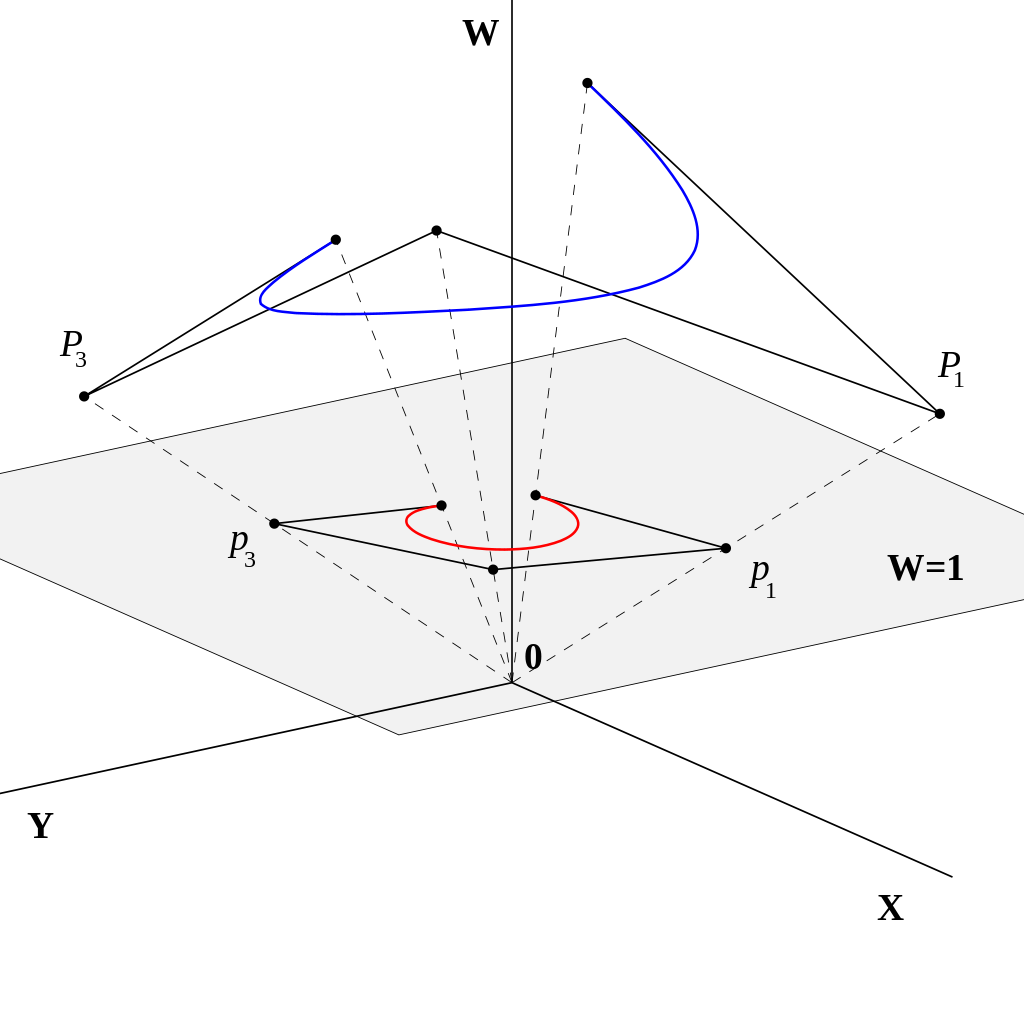
\includegraphics[width=.7\textwidth]{./pictures/RationalBezier_mapping.png}
\caption{Mapping bei homogenen Koordinaten}
\label{abb:maphomokoord}
\end{figure}

Bézier-Kurven können an diese Punkte entsprechend angepasst werden, sodass sie nicht erst zurückgemapped werden müssen, sondern direkt die gewichteten Punkte $P^{w}$ verwenden können.
\begin{equation}
C^{w}(u) = \sum_{i=0}^{n} B_{i,n}(u)*P_{i}^{w}
\end{equation}
Diese Formel hat die exakt gleiche Bedeutung wie die gebrochen rationalen Bézier-Kurven.
Der Beweis ist im Anhang vermerkt. 

\subsection{Tensor Produkt Oberflächen}
\label{sec:tensorproduktoberflaechen}

Wie der Name bereits andeutet, sind Bézier-Kurven nur Kurven.
Damit lassen sich noch keine Oberflächen oder Volumen-Körper darstellen. 
Dies ist mit \emph{Tensor Produkt Oberflächen} (im Weiteren TPO) möglich
Diese können sich wie Bézier-Kurven in zwei Richtungen vorgestellt werden. 
Diese TPOs werden durch das Symbol $S(u,v)$ dargestellt. 
Dabei sind $u$ und $v$ Elemente einer Fläche im Koordinaten-System. 
Über dieser Fläche wird die TBO abgebildet. 

\begin{equation}
S(u,v) = (x(u,v), y(u,v), z(u,v)) = \sum_{i=0}^{n} \sum_{j=0}^{m} f_{i}(u) * g_{j}(v) * b_{i,j} 
\end{equation}

Diese Gleichung kann auch als Matrix-Multiplikation verstanden werden. 
Statt mit $i$ und $j$ durch zu iterieren, kann eine $n X m$ ermittelt werden, welche in das Koordinaten-System eingetragen werden kann.
Dabei ist $[f_{i}(u)]^{T}$ ein Reihenvektor der Größe  $(1) X (n+1)$.
Dagegen ist $[g_{j}(u)]$ ein Spaltenvektor der Größe $(m+1) X (1)$.
Die Punkte $[b_{i,j}]$ sind bereits in einer Matrix der Größe $(n+1) X (m+1)$ angeordnet. 
Somit verändert sich die Gleichung wie folgt: 

\begin{equation}
S(u,v) = \sum_{i=0}^{n} \sum_{j=0}^{m} f_{i}(u) * g_{j}(v) * b_{i,j}  = [f_{i}(u)]^{T} * [b_{i,j}] * [g_{j}(u)]
\end{equation}

Wenn diese allgemeine Form der TPO mit Bézier-Kurven als $f_{i}(u)$ und $g_{j}(v)$ verwendet werden, kann nahezu jede Oberfläche dargestellt werden. 

\begin{equation}
S(u,v) = \sum_{i=0}^{n} \sum_{j=0}^{m} B_{i,n}(u) * B_{j,m} (v) * P_{i,j}
\end{equation}

Für gebrochen rationale Bézier-Kurven können erneut die homogenen Koordinaten verwendet werden, sodass folgende Gleichung entsteht. 

\begin{equation}
S^{w}(u,v) =  \sum_{i=0}^{n} \sum_{j=0}^{m} B_{i,n}(u) * B_{j,m} (v) * P^{w}_{i,j}
\end{equation}

Mit dieser Gleichung können alle Oberlfächen dargestellt werden. 
Jedoch bietet diese Gleichung das Problem, dass sie sehr schnell zu sehr hohen Graden (große $n$ und $m$) von Bézier-Kurven ausarten.
Dadurch ist die Berechnung sehr kompliziert und rechenintensiv. 
Eine Lösung dafür wird im folgenden Kapitel dargestellt. 

\section{Definition NURBS}
\label{sec:definitionnurbs}
\subsection{B-Splines}
\label{sec:bsplines}
Eine Möglichkeit Oberflächen mathematisch darzustellen ist mit den Bézier-Kurven und den Tensor Produkt Oberflächen gegeben.
Um diese zu optimieren, wird NURBS verwendet.
NURBS steht für \emph{non-uniform rational B-splines}.
Der Begriff \emph{rational}, bzw. auf Deutsch: \emph{gebrochen rational} wurde im Abschnitt \ref{sec:bezierkurven} dargestellt. 
Diese Funktionen können eine größere Vielfalt an Kurven darstellen. 

Wenn die deutsche Grammatik herangezogen wird, steht das Hauptwort eines zusammengesetzten Wortes am Schluss, weshalb der nächste zu betrachtende Bereich die \emph{B-Splines} sind. 
B-Splines sind Kurven oder Flächen, welche aus vielen einzelnen Kurven/Flächen bestehen. 
Dadurch gibt es keinen globalen Einfluss von Kontrollpunkten mehr, sondern nur noch einen lokalen. 
Wenn bei einem TPO ein Kontrollpunkt verändert wird, dann verändert sich an jedem Punkt der Oberfläche der Wert.
Wenn ein B-Spline aus verschiedenen unabhängigen Kurven aufgebaut ist, dann verändert sich bei einer Kontrollpunktänderung nur lokal die Kurve. 
Eine kontinuierliche Kurve wird garantiert, indem der letzte Punkt $P_{n}$ der vorhergehenden Kurve gleich dem ersten Punkt $P_{0}$. 

Eine Möglichkeit diese B-Splines darzustellen ist sind \emph{B-Spline Basis Funktionen} (Basisfunktionen). 
Diese werden im folgenden als rekursive Folge dargestellt.
Bei einer rekursiven Folge definiert sich ein Element $n$ aus vorangegangenen Elementen $n-k$.
Dabei ist $k$ eine positive natürliche Zahl mit $k \leq n$.

Die bekannteste rekursive Folge ist vermutlich die Fibonacci folge: $fib(n) = fib(n-1) + fib(n-2)$.
Dabei muss ein Anker defineirt werden.
Bei Fibonacci ist es: $fib(0) = fib(1) = 1$.

Die Basisfunktionen können wie folgt definiert werden:

\begin{equation}
N_{i,p}(u) = \frac{u-u_{i}}{u_{u+i}-u_{i}} * N_{i,p-1}(u) + \frac{u_{i+p+1} - u}{u_{i+p+1} - u_{i+1}} * N_{i+1,p-1}(u)
\end{equation}
Dabei ist der Anker für $p = 0$ definiert. 
\begin{equation}
N_{i,0}(u) = \Biggl\{ \substack{1 \text{ wenn } u_{i} \leq u_{i+1} \\ 0 \text{ wenn }sonst}\Biggr\}
\end{equation}

Dabei wird ein Knotenvektor $U = \{u_{0}, u_{1}, ..., u_{n}\}$ benötigt, welcher die \emph{Step-Funktionen} $N_{i,p}(u)$ ihren nicht-Null-Bereich definiert.
Dadurch ist die Lokalität möglich.
Die B-Spline Basisfunktionen können nur in den Bereich eine Wirkung auf die endgültige \emph{B-Spline}-Kurve haben, in welcher sie nicht Null sind. 
Dadurch ist eine Änderung im Bereich von $u_{i}$ bis $u_{i+1}$ nur durch die Basisfunktionen veränderbar, welche die Funktion $N_{i,0}(u)$ in ihrer Berechnung nutzen.

Wenn eine Basisfunktion berechnet wird, dann bildet sich eine Art Dreieck. 
Dabei ist die Basis des Dreiecks das $i$ und der Grad $p$ ist die Höhe des Dreiecks.

\begin{tabular}{c c c c c}
 &  & $N_{0,2}(u)$ &  &  \\
 & $N_{0,1}(u)$ &  & $N_{1,1}(u)$ &  \\
$N_{0,0}(u)$ &  & $N_{1,0}(u)$ &  & $N_{2,0}(u)$ \\
\end{tabular}

Die Anzahl der Basisfunktionen in jedem Grad nimmt ab, desto höher der Grad wird.
Somit ist auch nur ein maximaler Grad $p \leq n-1$ möglich.
Die Anzahl der Knoten im Knotenvektor
Es sind dabei $n-i$ Basisfunktionen mit dem Grad Null möglich.


\subsection{Eigenschaften von NURBS}
Zusammenfassend können NURBS-Kurven mit folgender Gleichung dargestellt werden. 
Dabei sind $\{P_{i}\}$ die Kontrollpunkte, welche durch die $\{w_{i}\}$ gewichtet werden.
Die B-Spline Basis-Funktionen sind durch $\{N_{i,p}(u)\}$ definiert.

\begin{equation}
C(u) = \frac{\sum_{i=0}^{n}N_{i,p}(u)*w_{i}*P_{i}}{\sum_{i=0}^{n}N_{i,p}(u)*w_{i}}
\end{equation}

Dabei können die gebrochen rationalen Basisfunktionen $R_{i,p}(u)$ herausgenommen werden, sodass darüber einige Eigenschaften abgeleitet werden können.

\begin{equation}
R_{i,p}(u) = \frac{N_{i,p}(u)*w_{i}}{\sum_{j=0}^{n}N_{j,p}(u)*w_{j}}
\end{equation}
\begin{equation}
C(u) = \sum_{i=0}^{n}R_{i,p}(u)*P_{i}
\end{equation}

Folgende Eigenschaften lassen sich auf diese gebrochen rationalen Basisfunktionen ableiten:

\subsubsection*{Nichtnegativ}
Es gilt:

\begin{equation}
\forall  u \in [0,1],  i,p : R_{i,p}(u) \geq 0
\end{equation}

Dies leitet sich aus der nichtnegativen Eigenschaft von $\{N_{i}(u)\}$ ab.
Alle $\{w_{i}\}$ müssen dahingehend immer positiv oder Null sein.

Somit hat jeder Punkt $\{P_{i}\}$ niemals einen abstoßenden Effekt auf die Kurve, solange die Gewichtung nicht negativ ist.

\subsubsection*{Teil eines Ganzes}
Es gilt:
\begin{equation}
\sum_{i=0}^{n}R_{i,p}(u) = 1; u \in [0,1]
\end{equation}

Im Zusammenhang mit der Nichtnegativität gilt, dass $0 \leq R_{i,p}(u) \leq 1$ gilt.

\subsubsection*{Anfang- und Endpunkt-Gleichheit}
Es gilt:
\begin{equation}
R_{0,p}(0) = R_{n,p}(1) = 1
\end{equation}

Dadurch werden am Ende die Kontrollpunkte $P_{0}$ und $P_{n}$ durch die Kurve geschnitten.
Den es gilt für die NURBS-Kurven:
\begin{equation}
C(0) = P_{0} ; C(1) = P_{n}
\end{equation}

In der Modellierung ist es dahingehend sinnvoll, wenn die Anfang- und Endpunkte auch den Anfang und das Ende des Modells darstellen.

\subsubsection*{Lokalität}
Eine Veränderung ändert immer nur einen fest abgegrenzten Bereich .
Dadurch ist eine komplexe Modellierung erst möglich.
Wenn also der Punkt $P_{i}$ oder die Gewichtung dieses Punktes verändert wird, ändert sich die Kurve nur im Bereich $[u_{i}, u_{i-1}]$.


\subsubsection*{Ableitungsregeln}
Es ist möglich, $R_{i,p}(u)$ an dem Knoten $u_{i}$ k-mal abzuleiten, wenn es keine Nullstelle ist.
Die Variable $k$ ist hierbei die Multiplizität des Knotens $u_{i}$.
Dadurch ist ein flüssiger Übergang zwischen den unterschiedlichen Knoten-Abschnitten möglich.

Bei einer NURBS Kurve ist es nicht mehr k-mal Ableitbar,  sondern $k-p$ mal ableitbar. 
Dabei ist $k$ wieder die Multiplizität des Knotens und $p$ der Grad.
Desto höher der Grad einer NURBS-Kurve ist, desto geringer ist die Kontinuität. 

\subsubsection*{Vereinfachung}
Wenn die Gewichtungen $\{w_{i}\}$ konstant sind, dann gilt:

\begin{equation}
R_{i,p}(u) = N_{i,p}(u)
\end{equation}

Dabei sind $\{N_{i,p}(u)\}$ die B-Spline Basis Funktionen. 
Somit kann der Rechenaufwand deutlich verringert werden, solange die Gewichtungen gleich sind.



\section{Modellierung}
\label{sec:modellierung}

\section{Fazit}
\label{sec:fazit}
\section{Anhang}
\subsection*{Umformung Bézier-Kurven mit $P_{i}^{w}$ auf Bézier-Kurven mit $w_{i}*P_{i}$}
\[C^{w}(u) = \sum_{i=0}^{n} B_{i,n} (u) * P^{w}_{i}\]
\[X(u) = \sum_{i=0}^{n} B_{i,n} (u) * w_{i} * x_{i}\]
\[Y(u) = \sum_{i=0}^{n} B_{i,n} (u) * w_{i} * y_{i}\]
\[Z(u) = \sum_{i=0}^{n} B_{i,n} (u) * w_{i} * z_{i}\]
\[W(u) = \sum_{i=0}^{n} B_{i,n} (u) * w_{i}\]

\[x(u) = \frac{X(u)}{W(u)} = \frac{\sum_{i=0}^{n} B_{i,n} (u) * w_{i} * x_{i}}{ \sum_{i=0}^{n} B_{i,n} (u) * w_{i}}\] 
\[y(u) = \frac{Y(u)}{W(u)} = \frac{\sum_{i=0}^{n} B_{i,n} (u) * w_{i} * y_{i}}{ \sum_{i=0}^{n} B_{i,n} (u) * w_{i}}\] 
\[z(u) = \frac{Z(u)}{W(u)} = \frac{\sum_{i=0}^{n} B_{i,n} (u) * w_{i} * z_{i}}{ \sum_{i=0}^{n} B_{i,n} (u) * w_{i}}\] 

\[C(u) = (x(u), y(u), z(u)) = \frac{\sum_{i=0}^{n} B_{i,n}(u) * w_{i} * (x_{i}, y_{i}, z_{i})}{\sum_{i=0}^{n} B_{i,n}(u) * w_{i}} =  \frac{\sum_{i=0}^{n} B_{i,n}(u) * w_{i} * P_{i}}{\sum_{i=0}^{n} B_{i,n}(u) * w_{i}}\]

\subsection*{B-Spline Basisfunktions Programm}

Mit \emph{jupyter-notebook} wurde das Programm ausgeführt, um die entsprechenden Bilder zu erzeugen. 
Die Variable $p$ anpassen, um den Grad zu ändern.
Die Liste $us$ anpassen, um den Knoten-Vektor zu ändern.

\begin{lstlisting}[caption=B-Splines Basisfunktionen, label=bsplineprogramm, language=Python]
import matplotlib.pyplot as plt

def bsplinebase(i,p,us,u):
    if p == 0:
        if u < us[i+1] and u >= us[i]:
            return 1
        else:
            return 0
    else:
        try:
            a = (u - us[i])/(us[i+p] - us[i]) * bsplinebase(i, p-1, us, u)
        except ZeroDivisionError:
            a = 0
        try:
            b = (us[i+p+1] - u)/(us[i+p+1] - us[i+1]) * bsplinebase(i+1, p-1, us, u)
        except:
            b = 0
        return a+b

us = [0,0,0,1,2,3,4,4,5,5,5]
p = 5

fig, ax = plt.subplots(ncols=1, figsize=(40, 5))

u = 0
a = [0]
xs = [0]

for i in range(0,10-p):
    while u < max(us)+ .1:
        xs.append(u)
        a.append(bsplinebase(i,p,us,u))
        u += 0.001
    u = 0
    ax.plot(xs,a)
    a = [0]
    xs = [0]
\end{lstlisting}
\end{document}